%%%%%%%%%%%%%%%%%%%%%%%%%%%%%%%%%%%%%%%%%
%  My documentation report
%  Objetive: Explain what I did and how, so someone can continue with the investigation
%
% Important note:
% Chapter heading images should have a 2:1 width:height ratio,
% e.g. 920px width and 460px height.
%
%%%%%%%%%%%%%%%%%%%%%%%%%%%%%%%%%%%%%%%%%


%----------------------------------------------------------------------------------------
%	PACKAGES AND OTHER DOCUMENT CONFIGURATIONS
%----------------------------------------------------------------------------------------

\documentclass[11pt,fleqn]{book} % Default font size and left-justified equations

\usepackage[top=3cm,bottom=3cm,left=3.2cm,right=3.2cm,headsep=10pt,letterpaper]{geometry} % Page margins

\usepackage{xcolor} % Required for specifying colors by name
\definecolor{ocre}{RGB}{52,177,201} % Define the orange color used for highlighting throughout the book

% Font Settings
\usepackage{avant} % Use the Avantgarde font for headings
%\usepackage{times} % Use the Times font for headings
\usepackage{mathptmx} % Use the Adobe Times Roman as the default text font together with math symbols from the Sym­bol, Chancery and Com­puter Modern fonts
\usepackage{microtype} % Slightly tweak font spacing for aesthetics
\usepackage[utf8]{inputenc} % Required for including letters with accents
\usepackage[T1]{fontenc} % Use 8-bit encoding that has 256 glyphs
\usepackage{amsthm}

% Bibliography
\usepackage[style=alphabetic,sorting=nyt,sortcites=true,autopunct=true,babel=hyphen,hyperref=true,abbreviate=false,backref=true,backend=biber]{biblatex}
\addbibresource{bibliography.bib} % BibTeX bibliography file
\defbibheading{bibempty}{}

\input{structure} % Insert the commands.tex file which contains the majority of the structure behind the template

%----------------------------------------------------------------------------------------
%	Definitions of new commands
%----------------------------------------------------------------------------------------

\def\R{\mathbb{R}}
\newcommand{\cvx}{convex}
\newcommand{\norm}[1]{\left\lVert#1\right\rVert}
\begin{document}

%----------------------------------------------------------------------------------------
%	TITLE PAGE
%----------------------------------------------------------------------------------------

\begingroup
\thispagestyle{empty}
\AddToShipoutPicture*{\put(0,0){\includegraphics[scale=1.25]{esahubble}}} % Image background
\centering
\vspace*{5cm}
\par\normalfont\fontsize{35}{35}\sffamily\selectfont
\textbf{Computational Biology 2021}\\
{\LARGE Expectation-Maximization of the PMF}\par % Book title
\vspace*{1cm}
{\Huge Technical Report}\par % Author name
\endgroup

%----------------------------------------------------------------------------------------
%	COPYRIGHT PAGE
%----------------------------------------------------------------------------------------

\newpage
~\vfill
\thispagestyle{empty}

%\noindent Copyright \copyright\ 2014 Andrea Hidalgo\\ % Copyright notice

\noindent \textsc{Biosystems Simulation Lab, National Chiao Tung University}\\

\noindent \textsc{github.com/yizaochen/emtheory}\\ % URL

\noindent This research was done under the supervision of Dr. Jhih-Wei Chu with the financial support of MOST Taiwan.\\ % License information

\noindent \textit{First release, November 2020} % Printing/edition date

%----------------------------------------------------------------------------------------
%	TABLE OF CONTENTS
%----------------------------------------------------------------------------------------

\chapterimage{head1.png} % Table of contents heading image

\pagestyle{empty} % No headers

\tableofcontents % Print the table of contents itself

%\cleardoublepage % Forces the first chapter to start on an odd page so it's on the right

\pagestyle{fancy} % Print headers again

%----------------------------------------------------------------------------------------
%	CHAPTER 1
%----------------------------------------------------------------------------------------
\chapterimage{head2.png} % Chapter heading image
\chapter{Langevin Dynamics}
\section{Basic Equation}
\begin{definition}
\begin{align}
        dx_t=D F(x_t)dt  + \sqrt{2D}d{W}_t.
\end{align}
\label{langevin}
\end{definition}

\subsection{The most disordered dynamics as reference}
\begin{align}
      V_{\rm ref}(x) &= 0\\
      F_{\rm ref}(x) &= 0\\
      D &= 4.845 \times 10^{9}~~\text{\AA}^2~s^{-1}  
\end{align}

\begin{center}
        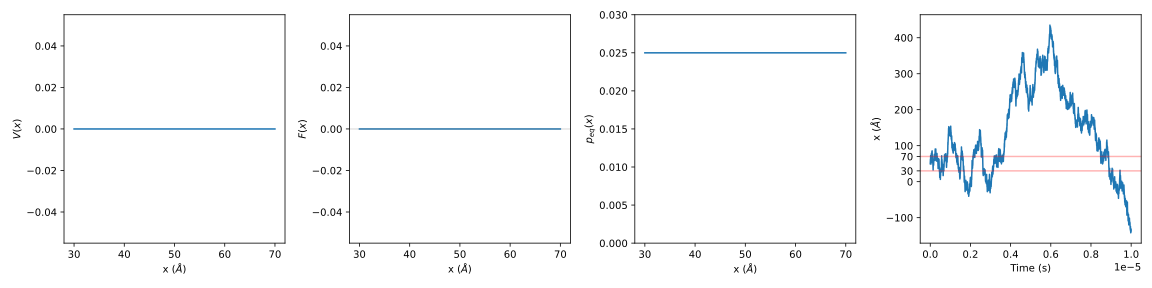
\includegraphics[scale=0.35]{ch1/zero_force_dynamic.pdf} 
\end{center}

\subsection{Harmonic Well}
\begin{align}
        V(x) &= k (x-50)^2\\
        F(x) &= 2k(x-50)  \\
        p_{\rm eq}(x) &= \exp{(-V(x))} \\
        D &= 4.845 \times 10^{9}~~\text{\AA}^2~s^{-1}
\end{align}
Here, $k=0.5$ kcal/mol/Å$^2$
\begin{center}
        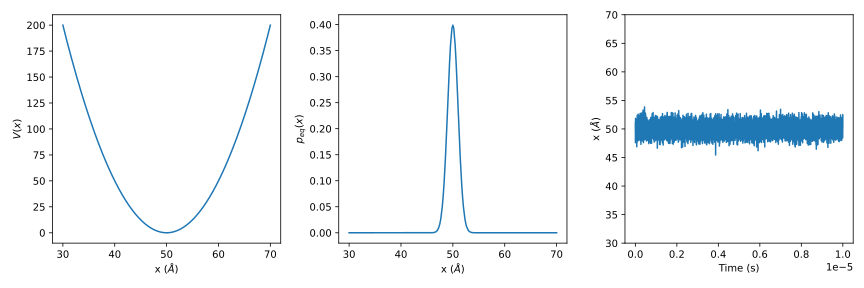
\includegraphics[scale=0.35]{ch1/single_well.pdf} 
\end{center}

\subsection{Double Well}
\begin{align}
        V(x) &= -\frac{1}{4} h^4 x^2 + \frac{1}{2} c^2 x^4 + d\\
        c    &= \sqrt{\frac{2H}{W^4}},H > 0 \\
        h    &= \sqrt{2Wc} \\
        F(x) &= \frac{1}{2} h^4 x - 2 c^2 x^3\\
        p_{\rm eq}(x) &= \exp{(-V(x))} \\
        D &= 4.845 \times 10^{9}~~\text{\AA}^2~s^{-1}\\
\end{align}
where $d$ is y-intercept, $H$ is the height of the central peak, and $W$ is the width between two valleys. In the following case, $H=5$ and $W=10$.
\begin{center}
        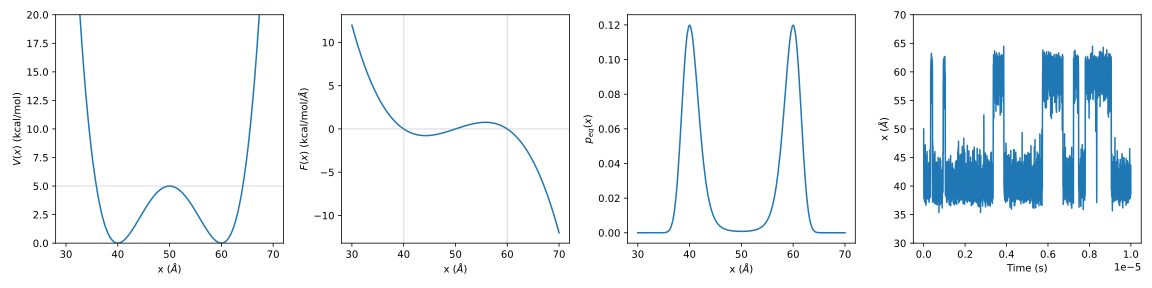
\includegraphics[scale=0.35]{ch1/double_well.pdf} 
\end{center}
%----------------------------------------------------------------------------------------
%	CHAPTER 2
%----------------------------------------------------------------------------------------
\chapterimage{head2.png} % Chapter heading image
\chapter{Bayesian Inference Framework}
\section{Graphical Model}
\begin{definition}
We denote a particular configuration as $(\textbf{x}, \textbf{y})$
\begin{equation}
(\textbf{x}, \textbf{y})=(x_0, x_1, \cdots, x_T, y_1, \cdots, y_T)
\end{equation}
\end{definition}

\begin{definition}[The joint probability]
\begin{equation}
p(\textbf{x}, \textbf{y})= p(x_0)\prod_{t=0}^{T-1} p(x_{t+1}|x_t) \prod_{t=0}^{T}p(y_t|x_t)
\end{equation}
\end{definition}
\begin{center}
        \includegraphics[scale=0.8]{ch2/four_states_ex.png}   
\end{center}

\section{Forward algorithm}
\subsection{Probability Meaning}
$ \left<\alpha_{t_{\tau}}|x \right>$ is the joint probability amplitude of emitting a partial sequence of outputs $(y_1,\cdots,y_{\tau})$ and ending up in state $x_{\tau}$. That is,
\begin{equation}
        (\left<\alpha_{t_{\tau}}|x \right>)^2 = p(y_1,\cdots,y_{\tau}, x_{\tau})
\end{equation}
For example, $(\left<\alpha_{t_2}|x \right>)^2 = p(y_1, y_2, x_2)$
\begin{center}
        \includegraphics[scale=0.8]{ch2/alpha_example.pdf}
\end{center}
\subsection{alpha-t0}
\begin{definition}[$\left< \hat{\alpha}_{t_0} \right|$]
Since there is no external forces, the initial state, $\left< \alpha_{t_0} \right|$, is assumed to follow the equilibrium distribution $\rho_{eq}(x)=\sqrt{p_{eq}(x)}$, that is
\begin{equation}
        \left< \alpha_{t_0} | x \right> = \rho_{eq}(x)
\end{equation}
\begin{center}
        \includegraphics[scale=0.45]{ch2/alpha_t0.png}   
\end{center}
And we know
\begin{align*}
        p(x,t=0) &= \rho_{eq}(x) \rho_{eq}(x)\\
        &= \rho_{eq}(x)[\left< \alpha_{t_0} | \psi_1 \right> \psi_1(x) + \left< \alpha_{t_0} | \psi_2 \right>\psi_2(x)+\cdots+\left< \alpha_{t_0} | \psi_{72} \right>\psi_{72}(x)]       
\end{align*}
where
\begin{align*}
        \left< \alpha_{t_0} | \psi_j \right> = \int w(x) \rho_{eq}(x) \psi_j(x) dx \approx \sum_{i=1}^{193} w(x_i) \rho_{eq}(x_i) \psi_j(x_i)
\end{align*}
$\left< \alpha_{t_0} \right|$ is a vector, which is shown in the right-bottom figure.
\begin{equation}
        \left< \alpha_{t_0} \right| = \begin{bmatrix}\left< \alpha_{t_0} | \psi_1 \right> & \left< \alpha_{t_0} | \psi_2 \right> & \cdots & \left< \alpha_{t_0} | \psi_{72} \right> \end{bmatrix}
\end{equation}
and the norm of $\left< \alpha_{t_0} \right|$ is defined by
\begin{align}
        \norm{\alpha_{t_0}} &=  \sqrt{\int w(x) (\left< \alpha_{t_0} | x_i \right>)^2 dx} \approx \sqrt{ \sum_{i=1}^{193} w(x_i) (\left< \alpha_{t_0} | x_i \right>)^2 } \\
        \norm{\alpha_{t_0}} &= \sqrt{(\left< \alpha_{t_0} | \psi_1 \right>)^2 + (\left< \alpha_{t_0} | \psi_2 \right>)^2 +\cdots + (\left< \alpha_{t_0} | \psi_{72} \right>)^2}
\end{align}
Furthermore, note that
\begin{equation}
        \left< \hat{\alpha}_{t_0} \right| = \frac{\left< \alpha_{t_{0}} \right|}{\norm{\alpha_{t_{0}}}} = \left< \alpha_{t_{0}} \right|
\end{equation}
because $\norm{\alpha_{t_0}} = 1$
\end{definition}

\begin{definition}[$\rho(x, t=\Delta t) = \left<\alpha_{t_0}| e^{-\textbf{H}\Delta t}|x \right>$]
\begin{align*}
        &p(x,t=\Delta t) = \rho_{eq}(x) \rho(x, \Delta t)\\
        &= \rho_{eq}(x)[ \left< \alpha_{t_0} | \psi_1 \right> e^{-\lambda_{1}\Delta t}\psi_1(x) + \cdots+ \left< \alpha_{t_0} | \psi_{72} \right> e^{(-\lambda_{72}\Delta t)}\psi_{72}(x)]  \\
        &=  \rho_{eq}(x)[ \left< \alpha_{t_0} | \psi_1 \right>\psi_1(x)+ \cdots + \left< \alpha_{t_0} | \psi_{72} \right> e^{(-\lambda_{72}\Delta t)}\psi_{72}(x)]  
\end{align*}
where $\lambda_1 = 0$
\begin{center}
        \includegraphics[scale=0.35]{ch2/alpha_t0_exp_dt.png}   
\end{center}
\end{definition}

\subsection{alpha-t1}
\begin{definition}[$\left< \hat{\alpha}_{t_1}\right|$]
\begin{equation}
        \left< \alpha_{t_1} \right| = \left< \alpha_{t_0} \right| e^{-\textbf{H} \Delta t} \textbf{y}_1     
\end{equation}
\begin{center}
        \includegraphics[scale=0.25]{ch2/photon_operator_y1.png}   
\end{center}
$\left< \alpha_{t_1} \right|$ carries "the joint probability amplitude" of observing all the photon data during $[0, t_1]$ and the system state at $t_1$, that is
\begin{equation}
        p(x, y_1) = (\left< \alpha_{t_1} | x \right>)^2
\end{equation}
We can do normalization to get $\left< \hat{\alpha}_{t_1} \right|$.
\begin{equation}
        \left< \hat{\alpha}_{t_1} \right| = \frac{\left< \alpha_{t_0} \right| e^{-\textbf{H}\Delta t} \textbf{y}_1}{\norm{\left< \alpha_{t_0} \right| e^{-\textbf{H}\Delta t} \textbf{y}_1}} = \frac{\left< \alpha_{t_{1}} \right|}{\norm{\alpha_{t_{1}}}}
\end{equation}
\begin{center}
        \includegraphics[scale=0.4]{ch2/alpha_1.png}   
\end{center}
$\left< \hat{\alpha}_{t_1} \right|$ is a probability amplitude, which square is 
\begin{align*}
        p(x | y_1) =  (\left< \hat{\alpha}_{t_1} | x \right>)^2
\end{align*}
Therefore
\begin{align*}
        \int p(x|y_1) dx \approx \sum_{k=1}^{193}w(x_k)(\left< \hat{\alpha}_{t_1} | x_k \right>)^2 &= 1 \\
        \norm{\hat{\alpha_{t_1}}} &= 1
\end{align*}
\end{definition}

\begin{definition}[$\left< \hat{\alpha}_{t_1}| e^{-\textbf{H}\Delta t} \right|$]
\begin{align*}
        \left< \hat{\alpha}_{t_1}| e^{-\textbf{H}\Delta t} \right| &= 
        \begin{bmatrix}
                \left< \hat{\alpha}_{t_1}| e^{-\textbf{H}\Delta t} | \psi_1 \right> &
                \left< \hat{\alpha}_{t_1}| e^{-\textbf{H}\Delta t} | \psi_2 \right> & 
                \cdots &
                \left< \hat{\alpha}_{t_1}| e^{-\textbf{H}\Delta t} | \psi_{72} \right>
        \end{bmatrix}\\
        &=
        \begin{bmatrix}
                e^{-\lambda_{1}\Delta t} \left< \hat{\alpha}_{t_1} | \psi_1 \right> &
                e^{-\lambda_{2}\Delta t} \left< \hat{\alpha}_{t_1} | \psi_2 \right> & 
                \cdots &
                e^{-\lambda_{72}\Delta t} \left< \hat{\alpha}_{t_1} | \psi_{72} \right> 
        \end{bmatrix}\\ 
        &=
        \begin{bmatrix}
                \left< \hat{\alpha}_{t_1} | \psi_1 \right> &
                e^{-\lambda_{2}\Delta t} \left< \hat{\alpha}_{t_1} | \psi_2 \right> & 
                \cdots &
                e^{-\lambda_{72}\Delta t} \left< \hat{\alpha}_{t_1} | \psi_{72} \right> 
        \end{bmatrix}
\end{align*}
The probability meaning is 
\begin{align*}
        (\left< \hat{\alpha}_{t_1}| e^{-\textbf{H}\Delta t} | x \right>)^2 = F(x_2) = p(x_1|y_1) p(x_2|x_1) 
\end{align*}
The case in our simulation, when $\Delta t = 10^{-9}$ s 
\begin{center}
        \includegraphics[scale=0.4]{ch2/alphat1_expdt_normalcase.png}   
\end{center}
In the right-bottom figure
\begin{align*}
        \int p(x_1|y_1)p(x_2|x_1)dx_2 = 0.326
\end{align*}
\end{definition}

\subsection{alpha-t2}
\begin{definition}[$\left< \hat{\alpha}_{t_2}\right|$]
\begin{equation}
        \left< \alpha_{t_2} \right| = \left< \alpha_{t_1} \right| e^{-\textbf{H}\Delta t} \textbf{y}_2     
\end{equation}
\begin{center}
        \includegraphics[scale=0.25]{ch2/photon_operator_y2.png}   
\end{center}
The probability meaning for $\left< \alpha_{t_2}\right|$ is 
\begin{align*}
        p(x_2, y_1, y_2) = (\left< \alpha_{t_2}| x \right>)^2
\end{align*}
and we can do normalization to get $\left< \hat{\alpha}_{t_2} \right|$, it has the information
\begin{equation}
        p(x|y_1,y_2) = (\left< \hat{\alpha}_{t_2} |x\right>)^2
\end{equation}
In detail
\begin{equation}
        \left< \hat{\alpha}_{t_2} \right| 
	= \frac{\left< \hat{\alpha}_{t_1} \right| e^{-\textbf{H}\Delta t} \textbf{y}_2}{\norm{\left< \hat{\alpha}_{t_1} \right| e^{-\textbf{H}\Delta t} \textbf{y}_2}} 
	= \frac{1}{\norm{\alpha_{t_{1}}}} \frac{\left< \alpha_{t_1} \right| e^{-\textbf{H}\Delta t} \textbf{y}_2}{\norm{\left< \hat{\alpha}_{t_1} \right| e^{-\textbf{H}\Delta t} \textbf{y}_2}} 
	= \frac{1}{\norm{\alpha_{t_{1}}}} \frac{1}{\norm{\left< \hat{\alpha}_{t_1} \right| e^{-\textbf{H}\Delta t} \textbf{y}_2}} \left< \alpha_{t_2} \right| 
	= \frac{1}{\norm{\alpha_{t_2}}} \left< \alpha_{t_2} \right|
\end{equation}
where
\begin{equation}
        \norm{\alpha_{t_2}} = \norm{\alpha_{t_{1}}} \norm{\left< \hat{\alpha}_{t_1} \right| e^{-\textbf{H}\Delta t} \textbf{y}_2} 
	= \norm{\left < \hat{\alpha}_{t_{0}} \right| e^{-\textbf{H}\Delta t} \textbf{y}_1} \norm{\left< \hat{\alpha}_{t_1} \right| e^{-\textbf{H}\Delta t} \textbf{y}_2}
\end{equation}
\begin{center}
        \includegraphics[scale=0.4]{ch2/alpha_2.png}   
\end{center}
\end{definition}

\begin{definition}[$\left< \hat{\alpha}_{t_2}| e^{-\textbf{H}\Delta t} \right|$]
The probability meaning is 
\begin{align*}
        (\left< \hat{\alpha}_{t_2}| e^{-\textbf{H}\Delta t} | x_3 \right>)^2 = \int p(x_2 | y_1, y_2) p(x_3|x_2) dx_3  
\end{align*}
\begin{center}
        \includegraphics[scale=0.4]{ch2/alphat2_expdt.png}   
\end{center}
\end{definition}

\subsection{alpha-t3}
\begin{definition}[$\left< \hat{\alpha}_{t_3}\right|$]
\begin{equation}
        \left< \alpha_{t_3} \right| = \left< \alpha_{t_2} \right| e^{-\textbf{H}\Delta t} \textbf{y}_3               
\end{equation}
\begin{center}
        \includegraphics[scale=0.25]{ch2/photon_operator_y3.png}   
\end{center}
\begin{equation}
        \left< \hat{\alpha}_{t_3} \right| 
	= \frac{\left< \hat{\alpha}_{t_2} \right| e^{-\textbf{H}\Delta t} \textbf{y}_3}{\norm{\left< \hat{\alpha}_{t_2} \right| e^{-\textbf{H}\Delta t} \textbf{y}_3}} 
	= \frac{1}{\norm{\alpha_{t_{2}}}} \frac{\left< \alpha_{t_2} \right| e^{-\textbf{H}\Delta t} \textbf{y}_3}{\norm{\left< \hat{\alpha}_{t_2} \right| e^{-\textbf{H}\Delta t} \textbf{y}_3}} 
	= \frac{1}{\norm{\alpha_{t_3}}} \left< \alpha_{t_3} \right|
\end{equation}
where
\begin{equation}
        \norm{\alpha_{t_3}} = \norm{\alpha_{t_{2}}} \norm{\left< \hat{\alpha}_{t_2} \right| e^{-\textbf{H}\Delta t} \textbf{y}_3} 
        = \norm{\left < \hat{\alpha}_{t_{0}} \right| e^{-\textbf{H}\Delta t} \textbf{y}_1} \norm{\left< \hat{\alpha}_{t_1} \right| e^{-\textbf{H}\Delta t} \textbf{y}_2} \norm{\left < \hat{\alpha}_{t_{2}} \right| e^{-\textbf{H}\Delta t} \textbf{y}_3}    
\end{equation}
\begin{center}
\includegraphics[scale=0.4]{ch2/alpha_3.png}
\end{center}
\end{definition}

\begin{definition}[$\left< \hat{\alpha}_{t_3}| e^{-\textbf{H}\Delta t} \right|$]
The probability meaning is 
\begin{align*}
        (\left< \hat{\alpha}_{t_3}| e^{-\textbf{H}\Delta t} | x_4 \right>)^2 = \int p(x_3 | y_1, y_2, y_3) p(x_4|x_3) dx_4  
\end{align*}
\begin{center}
        \includegraphics[scale=0.4]{ch2/alphat3_expdt.png}   
\end{center}
\end{definition}

\subsection{alpha-t4}
\begin{definition}[$\left< \hat{\alpha}_{t_4}\right|$]
\begin{equation}
        \left< \alpha_{t_4} \right| = \left< \alpha_{t_3} \right| e^{-\textbf{H}\Delta t} \textbf{y}_4
\end{equation}
\begin{center}
        \includegraphics[scale=0.25]{ch2/photon_operator_y4.png}   
\end{center}
\begin{equation}
        \left< \hat{\alpha}_{t_4} \right| 
	= \frac{\left< \hat{\alpha}_{t_3} \right| e^{-\textbf{H}\Delta t} \textbf{y}_4}{\norm{\left< \hat{\alpha}_{t_3} \right| e^{-\textbf{H}\Delta t} \textbf{y}_4}} 
        = \frac{1}{\norm{\alpha_{t_{3}}}} \frac{\left< \alpha_{t_3} \right| e^{-\textbf{H}\Delta t} \textbf{y}_4}{\norm{\left< \hat{\alpha}_{t_3} \right| e^{-\textbf{H}\Delta t} \textbf{y}_4}} 
        = \frac{1}{\norm{\alpha_{t_4}}} \left< \alpha_{t_4} \right|
\end{equation}
where
\begin{equation}
\begin{split}
        \norm{\alpha_{t_4}} &= \norm{\alpha_{t_{3}}} \norm{\left< \hat{\alpha}_{t_3} \right| e^{-\textbf{H}\Delta t} \textbf{y}_4}\\
        &= \norm{\left< \hat{\alpha}_{t_{0}} \right| e^{-\textbf{H}\Delta t} \textbf{y}_1} \norm{\left< \hat{\alpha}_{t_1} \right| e^{-\textbf{H}\Delta t} \textbf{y}_2} \norm{\left < \hat{\alpha}_{t_{2}} \right| e^{-\textbf{H}\Delta t} \textbf{y}_3} \norm{\left < \hat{\alpha}_{t_{3}} \right| e^{-\textbf{H}\Delta t} \textbf{y}_4}
\end{split}
\label{eq:alphat4}
\end{equation}
\begin{center}
        \includegraphics[scale=0.4]{ch2/alpha_4.png}
\end{center}
\end{definition}

\begin{definition}[$p(x_4|\textbf{y})$]
\begin{equation}
        \left(\left<  \hat{\alpha}_{t_4} | x \right>\right)^2 = p(x_4|y_1,y_2,y_3,y_4)
\end{equation}
\begin{center}
        \includegraphics[scale=0.7]{ch2/alpha_hat_4_graphical.pdf}
\end{center}
\begin{center}
        \includegraphics[scale=0.5]{ch2/posterior_4.png}
\end{center}       
\end{definition}

\section{Scaling Factor}
\begin{definition}[$\norm{\alpha_{t_{\tau}}}^2$]
\begin{equation}
        \left(\left< \hat{\alpha}_{t_{\tau}} | x \right>\right)^2 = p(x_{\tau}|y_1,\cdots,y_{\tau})  = 
        \frac{p(y_1,\cdots,y_{\tau}, x_{\tau})}{p(y_1,\cdots,y_{\tau})} =
        \frac{\left(\left< \alpha_{t_{\tau}} | x \right>\right)^2}{\norm{\alpha_{t_{\tau}}}^2} 
\end{equation}
Therefore,
\begin{equation}
        \norm{\alpha_{t_{\tau}}}^2 = p(y_1,\cdots,y_{\tau}) 
\end{equation}
\begin{center}
        \includegraphics[scale=0.6]{ch2/norm_example.pdf}
\end{center}
Furthermore, the likelihood function $p(\textbf{y})$
\begin{equation}
        \norm{\alpha_{t_{T}}}^2 =  p(y_1,\cdots,y_T) = p(\textbf{y})
\end{equation}
\end{definition}

\begin{definition}[Scaling factor $c_i$]
From eq(\ref{eq:alphat4}), we know
\begin{equation}
        \norm{\alpha_{t_{\tau}}} = \prod_{i=1}^{\tau} \norm{\left < \hat{\alpha}_{t_{i-1}} \right| e^{-\textbf{H}\Delta t} \textbf{y}_i} = \prod_{i=1}^{\tau} c_i
\end{equation}
To understand the probability meaning, we first do 
\begin{equation}
        \left(\left < \hat{\alpha}_{t_{i-1}} | e^{-\textbf{H}\Delta t} \textbf{y}_{i} | x \right>\right)^2 = p(x_{i},y_{i}|y_1,\cdots,y_{i-1})   
\end{equation}
\begin{equation}
\begin{split}       
        \norm{\left < \hat{\alpha}_{t_{i-1}} | e^{-\textbf{H}\Delta t} \textbf{y}_{i} \right|}^2 &= \int w(x) \left(\left < \hat{\alpha}_{t_{i-1}} | e^{-\textbf{H}\Delta t} \textbf{y}_{i} | x \right>\right)^2 dx \\
        &= \int p(x_{i},y_{i}|y_1,\cdots,y_{i-1}) dx = p(y_i | y_1,\cdots,y_{i-1})
\end{split}
\end{equation}
Therefore, the probability meaning of $c_i$ is 
\begin{equation}
        c_i^2 = p(y_i | y_1,\cdots,y_{i-1})
\label{eq:scalefactor} 
\end{equation}
Furthermore, the following is consistent
\begin{equation}
        \left(\left < \hat{\alpha}_{t_i} | x \right>\right)^2 =  p(x_{i}|y_1,\cdots,y_{i})  = 
        \frac{p(x_{i},y_{i}|y_1,\cdots,y_{i-1})}{p(y_i | y_1,\cdots,y_{i-1})} = \frac{  \left(\left < \hat{\alpha}_{t_{i-1}} | e^{-\textbf{H}\Delta t} \textbf{y}_{i} | x \right>\right)^2 }{ \norm{\left < \hat{\alpha}_{t_{i-1}} | e^{-\textbf{H}\Delta t} \textbf{y}_{i} \right|}^2 } 
\end{equation}
\end{definition}

\begin{definition}[Likelihood function]
The likelihood function $p(\textbf{y})$
\begin{equation}
        p(\textbf{y}) = p(y_1,\cdots,y_T) = \norm{\alpha_{t_{T}}}^2 = \prod_{i=1}^{T} \norm{\left < \hat{\alpha}_{t_{i-1}} \right| e^{-\textbf{H}\Delta t} \textbf{y}_i}^2 = \prod_{i=1}^{T} c_i^2
\end{equation}              
\end{definition}

\begin{definition}[Log likelihood function]
\begin{equation}
        l(\theta) = \ln{(p(\textbf{y}))} = \ln{(\prod_{i=1}^{T} c_i^2)} = 2\sum_{i=1}^{T} \ln{c_i}  
\end{equation}
\begin{center}
        \includegraphics[scale=0.45]{ch2/likelihood_example.png}
\end{center}
\end{definition}

\section{Backward algorithm}
\subsection{Probability Meaning}
First, the $ \left<x|\beta_{t_{\tau}} \right>$ is the probability amplitude of emitting a partial sequence of outputs $(y_{\tau+1},\cdots,y_{T})$ given that the system starts in state $x_{\tau}$. That is,
\begin{equation}
        (\left<x|\beta_{t_{\tau}} \right>)^2 = p(y_{\tau+1},\cdots,y_{T}|x_{\tau})
\end{equation}
For example, $(\left<x|\beta_{2} \right>)^2 = p(y_3, y_4|x_2)$
\begin{center}
        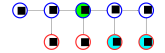
\includegraphics[scale=0.6]{ch2/beta_example.pdf}
\end{center}

\subsection{beta-4}
\begin{definition}[$\left | \beta_{t_4} \right > $]
As you can see in Definition(\ref{specialposterior}), we let
\begin{equation}\label{beta4}
        \left<x|\beta_{t_4} \right>=1~~\forall x 
\end{equation}
and we want to find $\left|\beta_{t_4} \right> $ which is in eigenspace
\begin{equation}
        \left|\beta_{t_4} \right> = \begin{bmatrix}
                \left< \psi_1|\beta_{t_4} \right> \\ \left< \psi_2|\beta_{t_4} \right> \\ \vdots \\ 
                \left< \psi_{72}|\beta_{t_4} \right>
        \end{bmatrix} 
\end{equation}
where
\begin{equation}\label{beta4dotproduct}
        \left< \psi_j | \beta_{t_4} \right> = \int w(x) \psi_j(x)  \left<x|\beta_{t_4} \right> dx
        = \int w(x) \psi_j(x) dx \approx \sum_{i=1}^{193} w(x_i) \psi_j(x_i).
\end{equation}
We substitute eq(\ref{beta4}) into eq(\ref{beta4dotproduct}).
\begin{center}
        \includegraphics[scale=0.45]{ch2/beta_4.png}
\end{center}
\end{definition}

\subsection{beta-3}
\begin{definition}[$ \left| \beta_{t_3} \right>$]
\begin{equation}
        \left|\beta_{t_3}  \right> =  \left| e^{-\textbf{H}\Delta t} \textbf{y}_4 |\beta_{t_4} \right>
\end{equation}
The probability meaning is
\begin{equation}
   \left( \left<x_3 |\beta_{t_3}  \right> \right)^2 = p(y_4 | x_3) = \int p(x_4 | x_3) p(y_4 | x_4) dx_4
\end{equation}
\begin{center}
        \includegraphics[scale=0.6]{ch2/beta_3_graphical.pdf}
\end{center}
\begin{center}
        \includegraphics[scale=0.45]{ch2/beta_3.png}
\end{center}
\end{definition}

\begin{definition}[$\left| \hat{\beta}_{t_3} \right>$]
\begin{equation}
        \left| \hat{\beta}_{t_{3}} \right> = \frac{ \left| \beta_{t_{3}} \right> }{ c_4 }
\end{equation}
where $c_4$ is the scaling factor computed in the forward part, as you can see in eq(\ref{eq:scalefactor}), and 
the probability meaning is
\begin{equation}
        \left(\left<x_3|\hat{\beta}_{t_{3}} \right>\right)^2 = \frac{p(y_4|x_3)}{p(y_4|y_1,y_2,y_3)} 
        =  \frac{ (\left<x_3|\beta_{t_{3}} \right>)^2 }{ c_4^2 }
\end{equation}
\begin{center}
        \includegraphics[scale=0.45]{ch2/beta_3_hat.png}
\end{center}
\begin{equation}
        p(x_3|\textbf{y}) = (\left<\hat{\alpha}_{t_{3}}|x \right>)^2 \left(\left<x|\hat{\beta}_{t_{3}} \right>\right)^2
\end{equation} 
\end{definition}

\subsection{beta-2}
\begin{definition}[$\left| \beta_{t_2} \right>$]
\begin{equation}
        \left|\beta_{t_2}  \right> =  \left| e^{-\textbf{H}\Delta t} \textbf{y}_3 |\beta_{t_3} \right>
\end{equation}
The probability meaning is
\begin{equation}
           \left( \left<x_2 |\beta_{t_2}  \right> \right)^2 = p(y_3, y_4 | x_2)
\end{equation}
\begin{center}
        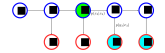
\includegraphics[scale=0.6]{ch2/beta_2_graphical.pdf}
\end{center}       
\end{definition}

\begin{definition}[$\left| \hat{\beta}_{t_2} \right>$]
\begin{equation}
        \left|\hat{\beta}_{t_2}  \right> =  \frac{\left| e^{-\textbf{H}\Delta t} \textbf{y}_3 |\hat{\beta}_{t_3} \right>}{c_3}
\end{equation}
where $c_3$ is the scaling factor computed in the forward part, as you can see in eq(\ref{eq:scalefactor}), and 
the probability meaning is
\begin{equation}
        \left(\left<x_2|\hat{\beta}_{t_{2}} \right>\right)^2 = \frac{p(y_3, y_4|x_2)}{p(y_3|y_1,y_2)} 
        =  \frac{ (\left<x_2|\beta_{t_{2}} \right>)^2 }{ c_3^2 }
\end{equation}
\begin{center}
        \includegraphics[scale=0.45]{ch2/beta_2_hat.png}
\end{center}
\begin{equation}
        p(x_2|\textbf{y}) = (\left<\hat{\alpha}_{t_{2}}|x \right>)^2 \left(\left<x|\hat{\beta}_{t_{2}} \right>\right)^2
\end{equation} 
\end{definition}

\subsection{beta-1}
\begin{definition}[$\left| \beta_{t_1} \right>$]
\begin{equation}
        \left|\beta_{t_1}  \right> =  \left| e^{-\textbf{H}\Delta t} \textbf{y}_2 |\beta_{t_2} \right>
\end{equation}
The probability meaning is
\begin{equation}
           \left( \left<x_1 |\beta_{t_1}  \right> \right)^2 = p(y_2, y_3, y_4 | x_1)
\end{equation}
\begin{center}
        \includegraphics[scale=0.6]{ch2/beta_1_graphical.pdf}
\end{center}       
\end{definition}

\begin{definition}[$\left| \hat{\beta}_{t_1} \right>$]
\begin{equation}
        \left|\hat{\beta}_{t_1}  \right> =  \frac{\left| e^{-\textbf{H}\Delta t} \textbf{y}_2 |\hat{\beta}_{t_2} \right>}{c_2}
\end{equation}
where $c_2$ is the scaling factor computed in the forward part, as you can see in eq(\ref{eq:scalefactor}), and 
the probability meaning is
\begin{equation}
        \left(\left<x_1|\hat{\beta}_{t_1} \right>\right)^2 = \frac{p(y_2, y_3, y_4|x_1)}{p(y_2|y_1)} 
        =  \frac{ (\left<x_1|\beta_{t_1} \right>)^2 }{ c_2^2 }
\end{equation}
\begin{center}
        \includegraphics[scale=0.45]{ch2/beta_1_hat.png}
\end{center}
\begin{equation}
        p(x_1|\textbf{y}) = (\left<\hat{\alpha}_{t_{1}}|x \right>)^2 \left(\left<x|\hat{\beta}_{t_{1}} \right>\right)^2
\end{equation} 
\end{definition}

\section{Posterior probability}
\begin{definition}[$p(x_{\tau}|\textbf{y})$] 
The posterior probability on a particular state node $x_{\tau}$, where $\textbf{y}$ is all emission sequence
\begin{align*}
        \textbf{y} = (y_1,\cdots,y_T)
\end{align*} 
\end{definition}
\noindent We focus on a particular state node $x_{\tau}$ and ask to calculate its posterior probability, $p(x_{\tau}| \textbf{y})$. And by Bayes' theorem,
\begin{equation}
p(x_{\tau} | \textbf{y}) = \frac{p(\textbf{y}|x_{\tau}) p(x_{\tau})}{p(\textbf{y})}
\end{equation}
Then, conditioning on $x_{\tau}$ and use conditional independence:
\begin{equation}
p(x_{\tau} | \textbf{y}) = \frac{p(y_1,\cdots,y_{\tau}|x_{\tau}) p(y_{\tau+1},\cdots,y_T|x_{\tau}) p(x_{\tau})}{p(\textbf{y})}
\end{equation}
Regroup the terms
\begin{equation}
\begin{split}
p(x_{\tau} | \textbf{y}) &= \frac{p(y_1,\cdots,y_{\tau},x_{\tau}) p(y_{\tau+1},\cdots,y_T|x_{\tau})}{p(\textbf{y})}\\
&=\frac{(\left<\alpha_{t_{\tau}}|x \right>)^2 (\left<x|\beta_{t_{\tau}} \right>)^2 }{p(\textbf{y})}
\end{split}
\end{equation}

\begin{definition}[Special case: $p(x_T|\textbf{y})$]
\label{specialposterior}
\begin{equation}
p(x_T | \textbf{y}) =\frac{(\left<\alpha_{t_T}|x \right>)^2 (\left<x|\beta_{t_T} \right>)^2 }{p(\textbf{y})}
\end{equation}
where
\begin{align}
        (\left<\alpha_{t_T}|x \right>)^2 &=  p(y_1,\cdots,y_T,x_T) = p(\textbf{y}, x_T) \\
        (\left<x|\beta_{t_T} \right>)^2 &= p(y_{T+1}|x_T)\text{~~~Some problem here!}
\end{align}
As you can see, we can not define $\left<x|\beta_{t_T} \right>$ because there is no $y_{T+1}$. Also, we notice
\begin{align*}
        p(x_T | \textbf{y}) = \frac{(\left<\alpha_{t_T}|x \right>)^2}{p(\textbf{y})} = \frac{p(\textbf{y}, x_T)}{p(\textbf{y})}
\end{align*}
Therefore, we just let
\begin{equation}
        \left<x|\beta_{t_T} \right>=1~~\forall x
\end{equation}
\end{definition}

\begin{definition}[$p(x_3|\textbf{y})$]
\begin{equation}
        p(x_3|\textbf{y}) = \frac{(\left<\alpha_{t_{3}}|x \right>)^2 (\left<x|\beta_{t_{3}} \right>)^2 }{p(\textbf{y})} 
        = (\left<\hat{\alpha}_{t_{3}}|x \right>)^2 \left(\left<x|\hat{\beta}_{t_{3}} \right>\right)^2
\end{equation}
where
\begin{equation}
        (\left<\hat{\alpha}_{t_{3}}|x \right>)^2 = 
        \frac{p(y_1,y_2,y_3, x_3)}{p(y_1,y_2,y_3)} =
        p(x_3|y_1,y_2,y_3)=
        \frac{\left(\left< \alpha_{t_3} | x \right>\right)^2}{\norm{\alpha_{t_3}}^2}   
\end{equation}
and
\begin{equation}
        \left(\left<x|\hat{\beta}_{t_{3}} \right>\right)^2 = \frac{p(y_4|x_3)}{p(y_4|y_1,y_2,y_3)} 
        =  \frac{ (\left<x|\beta_{t_{3}} \right>)^2 }{ c_4^2 }
\end{equation}
In the last line, we used eq(\ref{eq:scalefactor}).
\begin{center}
        \includegraphics[scale=0.6]{ch2/posterior_3.pdf}
\end{center}   
\end{definition}
%----------------------------------------------------------------------------------------
%	CHAPTER 3
%----------------------------------------------------------------------------------------
\chapterimage{head2.png} % Chapter heading image
\chapter{Spectral Finite Element Method}
\section{Domain of sFEM}
The grid size is 0.6250 Å. (The distance between two red points). Totally, there are 193 points.
\begin{center}
        \includegraphics[scale=0.3]{ch3/node.pdf}
\end{center}
\begin{itemize}
        \item The number of spectral element, $N_h=64$
        \item The order of interpolation polynomial, $N_p=4$
\end{itemize}
Therefore, we now have $V$, a vector space  of dimension $193$. This vector space has a natural basis, or we called it the standard basis
\begin{equation}
        \{\textbf{e}_1, \textbf{e}_2, ..., \textbf{e}_{193}\}
\end{equation}
where
\begin{equation}
\textbf{e}_1=  \begin{bmatrix} 1 \\ 0 \\ \vdots \\ 0 \end{bmatrix}~~
\textbf{e}_2=  \begin{bmatrix} 0 \\ 1 \\ \vdots \\ 0 \end{bmatrix}~~
\cdots ~~
\textbf{e}_{193} = \begin{bmatrix} 0 \\ 0 \\ \vdots \\ 1 \end{bmatrix} 
\end{equation}

\section{Weight function, orthogonality and norm}
\begin{definition}[inner product]
By using integral calculus, it is common to use the following to define the inner product of two functions $f$ and $g$ with respect to a nonnegative weight function $w$ over an interval $[a, b]$:
\begin{equation}
        \langle f, g\rangle_w = \int_a^b f(x)g(x)w(x)\,dx \approx \sum_{i=1}^{193}w(x_i)f(x_i)g(x_i) 
\end{equation}
\end{definition}

\begin{definition}[weight function $w(x)$]
From the  Gauss-Lobatto quadrature, we have
\begin{center}
        \includegraphics[scale=0.35]{ch3/weight_function.png}   
\end{center}
\end{definition}

\begin{definition}[Orthogonal]
We say that functions $f$ and $g$ are orthogonal if their inner product (equivalently, the value of this integral) is zero:
\begin{equation}
        \langle f,g\rangle _{w}=0.
\end{equation}
\end{definition}

\begin{definition}[Norm]
We define the norm with respect to this inner product as
\begin{equation}
        \|f\|_w = \sqrt{\langle f, f\rangle_w}
\end{equation}
\end{definition}

\section{Diagonalization of the operator}
\begin{definition}[Basis functions]
\begin{align}
        \psi^0_i(x) &= \rho_{\rm eq}(x) \phi^0_i(x) \\
        \phi^0_i(x) &= \sum_n c^0_n u_n(x).
\end{align}
\label{basisfunctions}
\end{definition}

\begin{definition}[Eigenvector matrix]
\begin{equation}
\Psi=
\begin{bmatrix}
\vert & \vert &  & \vert \\
\psi_1(x) & \psi_2(x) & \cdots & \psi_{N_v}(x) \\
\vert & \vert &  & \vert 
\end{bmatrix}
\end{equation}
\label{eigenvectormatrix}
Here, we get a set of orthonormal basis, $\langle \psi_i |$. The left part in the following part is 
\begin{equation}
        \Psi^T_{72\times 193}\Psi_{193 \times 72} = (\Psi^T\Psi)_{72 \times 72}
\end{equation}
The completeness relationship is actually can be seen by the blue points in the right part:
\begin{equation}
        \langle \psi_i(x),\psi_i(x)\rangle _{w} = \sum_{j=1}^{193}w(x_j)\psi_i(x_j)\psi_i(x_j)  = 1
\end{equation}
\begin{center}
        \includegraphics[scale=0.4]{ch3/eigenvec_matrix_complete.png}   
\end{center}
\end{definition}


%----------------------------------------------------------------------------------------
%	CHAPTER 4
%----------------------------------------------------------------------------------------
\chapterimage{head2.png} % Chapter heading image
\chapter{EM Algorithm}

\section{The General EM Algorithm}
\begin{definition}[The joint probability]
    \begin{equation}
        p(\textbf{x}, \textbf{y})= p(x_0)\prod_{t=1}^{T} p(x_{t}|x_{t-1}) p(y_t|x_t)
    \end{equation}
    \begin{center}
        \includegraphics[scale=0.6]{ch2/four_states_ex.png}   
    \end{center}
In this example
    \begin{equation}
    \begin{split}
        p(\textbf{x}, \textbf{y})= &[p(x_0) p(x_1|x_0) p(y_1|x_1)] [p(x_2|x_1) p(y_2|x_2)]  [p(x_3|x_2) p(y_3|x_3)] \\
        &[p(x_4|x_3) p(y_4|x_4)]
    \end{split}
    \end{equation}
\end{definition}

\begin{definition}[The likelihood functional]
\begin{equation}
    L[\theta] = p(\textbf{y};\theta) = \int d\textbf{x}p(\textbf{x}, \textbf{y})
\end{equation}
\end{definition}

\begin{definition}[The log-likelihood functional]
\begin{equation}
    l[\theta] = \ln{(\int d\textbf{x}p(\textbf{x}, \textbf{y}))}
\end{equation}
\end{definition}

\begin{definition}[Solve Euler-Lagrange equation]
Maximization for the optimal parameter set requires taking derivatives of the log-likelihood functional and solves the resulting Euler-Lagrange equation:
\begin{equation}
        \frac{\partial l[\theta]}{\partial \theta} = \frac{\partial}{\partial \theta} \ln{(\int d\textbf{x}p(\textbf{x}, \textbf{y}))} = 0
\end{equation}
We can further get
\begin{equation}
    \frac{\partial l[\theta]}{\partial \theta} =  \frac{\partial \ln{L[\theta]}}{\partial \theta} = \frac{1}{L[\theta]}\frac{\partial L[\theta]}{\partial \theta}
\end{equation}
Because we need to do maximization according to previous step($k$), we want to solve the
following equation
\begin{equation}
    0 = \frac{\partial l^k[\theta]}{\partial \theta} = \frac{1}{L^k[\theta]}\frac{\partial L^k[\theta]}{\partial \theta}
\end{equation}
And we can express the likelihood functional as
\begin{equation}
    L^k[\theta] = p(\textbf{y}) = \sum_{\tau=0}^{T-1} \left<\alpha^k_{t_{\tau}}\right|  e^{-\textbf{H} \Delta t} \left|\beta^k_{t_{\tau+1}}\right>
\end{equation}
Therefore, the maximization problem becomes to solve
\begin{equation}
    0 =  \frac{\partial l^k[\theta]}{\partial \theta} = \frac{1}{L^k[\theta]} \sum_{\tau=0}^{T-1} \frac{\partial}{\partial \theta} \left<\alpha^k_{t_{\tau}}\right|  e^{-\textbf{H} \Delta t} \left|\beta^k_{t_{\tau+1}}\right>
\end{equation}
\end{definition}

\section{The expected log of the complete likelihood}
\begin{definition}[$\left<\alpha^k_{t_{0}}\right|  e^{-\textbf{H} \Delta t} \left|\beta^k_{t_{1}}\right>$]
\begin{equation}
    \left< \alpha_{t_0} | e^{-\textbf{H}\Delta t} | \beta_{t_1} \right> = \int p(x_0) p(x_1|x_0) p(y_2,y_3,y_4|x_1) dx_1= p(x_0,y_2,y_3,y_4)
\end{equation}
    \begin{center}
        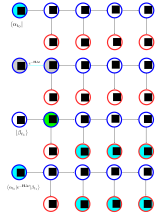
\includegraphics[scale=0.25]{ch4/alpha_t0_e_beta_t1.pdf}   
    \end{center}
\end{definition}

\begin{definition}[$\left<\alpha^k_{t_{1}}\right|  e^{-\textbf{H} \Delta t} \left|\beta^k_{t_{2}}\right>$]
\begin{equation}
    \left< \alpha_{t_1} | e^{-\textbf{H}\Delta t} | \beta_{t_2} \right> = \int p(x_1,y_1) p(x_2|x_1) p(y_3,y_4|x_2) dx_2= p(x_1,y_1,y_3,y_4)
\end{equation}
\begin{center}
    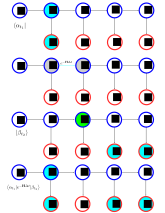
\includegraphics[scale=0.35]{ch4/alpha_t1_e_beta_t2.pdf}   
\end{center}
\end{definition}

\begin{definition}[$\left<\alpha^k_{t_{2}}\right|  e^{-\textbf{H} \Delta t} \left|\beta^k_{t_{3}}\right>$]
\begin{equation}
    \left< \alpha_{t_2} | e^{-\textbf{H}\Delta t} | \beta_{t_3} \right> = \int p(x_2,y_1,y_2) p(x_3|x_2) p(y_4|x_3) dx_3= p(x_2,y_1,y_2,y_4)
\end{equation}
\begin{center}
    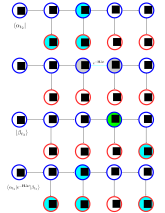
\includegraphics[scale=0.35]{ch4/alpha_t2_e_beta_t3.pdf}   
\end{center}
\end{definition}

\begin{definition}[$\left<\alpha^k_{t_{3}}\right|  e^{-\textbf{H} \Delta t} \left|\beta^k_{t_{4}}\right>$]
\begin{equation}
    \left< \alpha_{t_3} | e^{-\textbf{H}\Delta t} | \beta_{t_4} \right> = \int p(x_3,y_1,y_2,y_3) p(x_4|x_3) dx_4= p(x_3,y_1,y_2,y_3)
\end{equation}
\begin{center}
    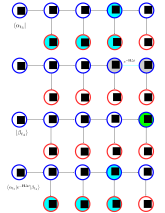
\includegraphics[scale=0.25]{ch4/alpha_t3_e_beta_t4.pdf}   
\end{center}
\end{definition}

\section{Update the equilibrium probability density}
\begin{definition}
    The basis functions in Def.(\ref{basisfunctions}) were used to update
\begin{align}
    p_{\rm eq}^{k+1}(x) &=\mathbb{E}^k_{X|Y} \left[ \delta(x-X) \right] \\
    &= p^k_{\rm{eq}}(x) \sum_{i,j} \mathbb{E}^k_{X|Y}[a_ib_j] \phi_i(x)\phi_j(x) \\
    &= \sum_{i,j} \psi_i(x) \mathbb{E}^k_{X|Y}[a_ib_j] \psi_j(x).
\end{align}
\end{definition}

\begin{definition}[Update from matrix multiplication]
\begin{align}
    p_{\rm eq}^{k+1}(x) = \mathrm{diag}(\Psi \mathbb{E}^k_{X|Y}[a_ib_j] \Psi^{\dagger})
\end{align}
\end{definition}

\begin{example}[$N_v=3$] In the matrix multiplication, I abbreviate $\mathbb{E}^k_{X|Y}[a_ib_j]$ as $a_ib_j$, and the grids are set like the bottom figure. We will show
\begin{align*}
    p_{\rm eq}^{k+1}(x) &=\sum_{i,j} \psi_i(x) \mathbb{E}^k_{X|Y}[a_ib_j] \psi_j(x) \\
    &= \mathrm{diag}(\Psi \mathbb{E}^k_{X|Y}[a_ib_j] \Psi^{\dagger})
\end{align*}
\begin{center}
    \includegraphics[scale=1.5]{ch4/ex1_grids.pdf}   
\end{center}
\begin{align*} 
&\Psi \mathbb{E}^k_{X|Y}[a_ib_j] \Psi^{\dagger} = \\
&\begin{bmatrix}
    \psi_1(x_1) & \psi_2(x_1) & \psi_3(x_1)  \\
    \psi_1(x_2) & \psi_2(x_2) & \psi_3(x_2) \\
    \psi_1(x_3) & \psi_2(x_3) & \psi_3(x_3)  \\
    \psi_1(x_4) & \psi_2(x_4) & \psi_3(x_4)  \\
    \psi_1(x_5) & \psi_2(x_5) & \psi_3(x_5)  
\end{bmatrix}
\begin{bmatrix}
    a_1 b_1 & a_1 b_2 & a_1 b_3  \\
    a_2 b_1 & a_2 b_2 & a_2 b_3 \\
    a_3 b_1 & a_3 b_2 & a_3 b_3
\end{bmatrix}
\begin{bmatrix}
    \psi_1(x_1) & \psi_1(x_2) & \psi_1(x_3) & \psi_1(x_4) & \psi_1(x_5) \\
    \psi_2(x_1) & \psi_2(x_2) & \psi_2(x_3) & \psi_2(x_4) & \psi_2(x_5) \\
    \psi_3(x_1) & \psi_3(x_2) & \psi_3(x_3) & \psi_3(x_4) & \psi_3(x_5) 
\end{bmatrix} \\
&=\begin{bmatrix}
    \sum_{i=1}^{3}a_i b_1 \psi_i(x_1) & \sum_{i=1}^{3}a_i b_2 \psi_i(x_1) & \sum_{i=1}^{3}a_i b_3 \psi_i(x_1) \\
    \sum_{i=1}^{3}a_i b_1 \psi_i(x_2) & \sum_{i=1}^{3}a_i b_2 \psi_i(x_2) & \sum_{i=1}^{3}a_i b_3 \psi_i(x_2) \\
    \sum_{i=1}^{3}a_i b_1 \psi_i(x_3) & \sum_{i=1}^{3}a_i b_2 \psi_i(x_3) & \sum_{i=1}^{3}a_i b_3 \psi_i(x_3) \\
    \sum_{i=1}^{3}a_i b_1 \psi_i(x_4) & \sum_{i=1}^{3}a_i b_2 \psi_i(x_4) & \sum_{i=1}^{3}a_i b_3 \psi_i(x_4) \\
    \sum_{i=1}^{3}a_i b_1 \psi_i(x_5) & \sum_{i=1}^{3}a_i b_2 \psi_i(x_5) & \sum_{i=1}^{3}a_i b_3 \psi_i(x_5) 
\end{bmatrix}\\
&\begin{bmatrix}
    \psi_1(x_1) & \psi_1(x_2) & \psi_1(x_3) & \psi_1(x_4) & \psi_1(x_5) \\
    \psi_2(x_1) & \psi_2(x_2) & \psi_2(x_3) & \psi_2(x_4) & \psi_2(x_5) \\
    \psi_3(x_1) & \psi_3(x_2) & \psi_3(x_3) & \psi_3(x_4) & \psi_3(x_5) 
\end{bmatrix}\\
&=
\begin{bmatrix}
\sum_{j=1}^{3} b_j \psi_j(x_1) \sum_{i=1}^{3}a_i \psi_i(x_1) &  \sum_{j=1}^{3} b_j \psi_j(x_2) \sum_{i=1}^{3}a_i \psi_i(x_1) &
\cdots & \sum_{j=1}^{3} b_j \psi_j(x_5) \sum_{i=1}^{3}a_i \psi_i(x_1) \\
\sum_{j=1}^{3} b_j \psi_j(x_1) \sum_{i=1}^{3}a_i \psi_i(x_2) &  \sum_{j=1}^{3} b_j \psi_j(x_2) \sum_{i=1}^{3}a_i \psi_i(x_2) &
\cdots & \sum_{j=1}^{3} b_j \psi_j(x_5) \sum_{i=1}^{3}a_i \psi_i(x_2) \\
\sum_{j=1}^{3} b_j \psi_j(x_1) \sum_{i=1}^{3}a_i \psi_i(x_3) &  \sum_{j=1}^{3} b_j \psi_j(x_2) \sum_{i=1}^{3}a_i \psi_i(x_3) &
\cdots & \sum_{j=1}^{3} b_j \psi_j(x_5) \sum_{i=1}^{3}a_i \psi_i(x_3) \\
\sum_{j=1}^{3} b_j \psi_j(x_1) \sum_{i=1}^{3}a_i \psi_i(x_4) &  \sum_{j=1}^{3} b_j \psi_j(x_2) \sum_{i=1}^{3}a_i \psi_i(x_4) &
\cdots & \sum_{j=1}^{3} b_j \psi_j(x_5) \sum_{i=1}^{3}a_i \psi_i(x_4) \\
\sum_{j=1}^{3} b_j \psi_j(x_1) \sum_{i=1}^{3}a_i \psi_i(x_5) &  \sum_{j=1}^{3} b_j \psi_j(x_2) \sum_{i=1}^{3}a_i \psi_i(x_5) &
\cdots & \sum_{j=1}^{3} b_j \psi_j(x_5) \sum_{i=1}^{3}a_i \psi_i(x_5)
\end{bmatrix}
\end{align*}
\end{example}

\section{EM Test}
\begin{center}
    \includegraphics[scale=0.36]{ch4/forward_backward_v2.png}   
\end{center}

\subsection{Initial Guess Test}
\begin{center}
    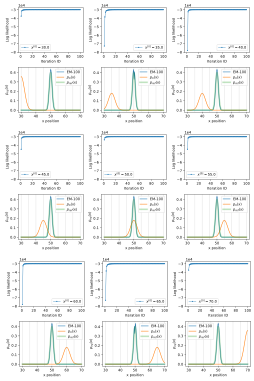
\includegraphics[scale=0.55]{ch4/initial_guess_test.pdf}   
\end{center}

\subsection{Troubleshooting: Double Peak}
\begin{center}
    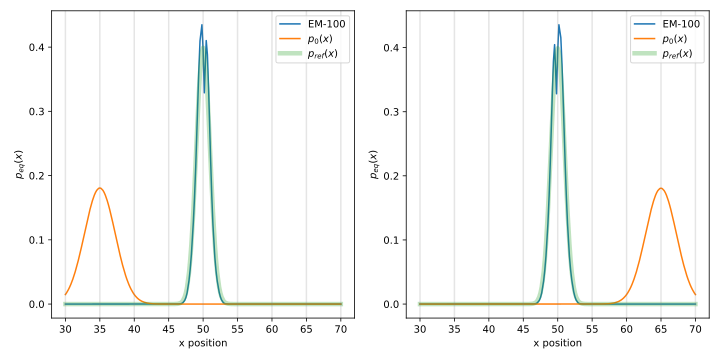
\includegraphics[scale=0.55]{ch4/double_peak_problem.pdf}   
\end{center}
\subsubsection{Step 1: Detect abrupt change}
\begin{itemize}
    \item Use finite difference to get $\frac{d p^{[k]}_{eq}(x)}{dx}$ and $\frac{d^2 p^{[k]}_{eq}(x)}{dx^2}$
    \item If $|\frac{d^2 p_{eq}(x)}{dx^2}|>1$, put the point into the list storing "change points"
    \item If $\text{Number}(\text{Change points}) > 0$, do smoothing. Else: no smooth 
\end{itemize}
\begin{center}
    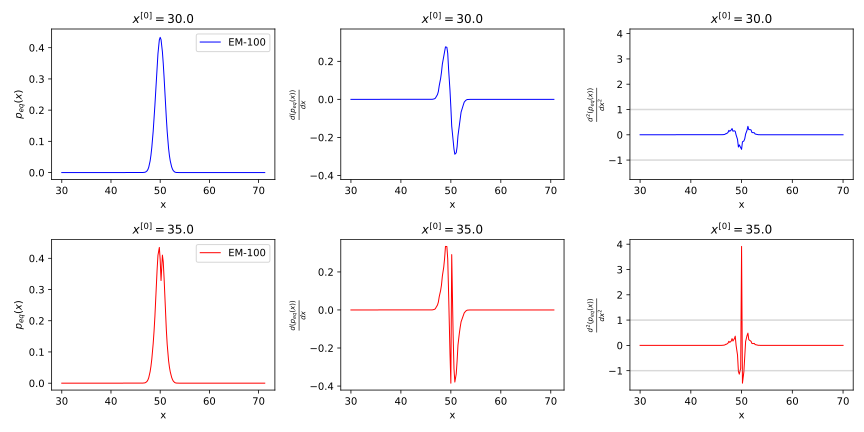
\includegraphics[scale=0.4]{ch4/double_peak_problem_derivative.pdf}   
\end{center}
\begin{center}
    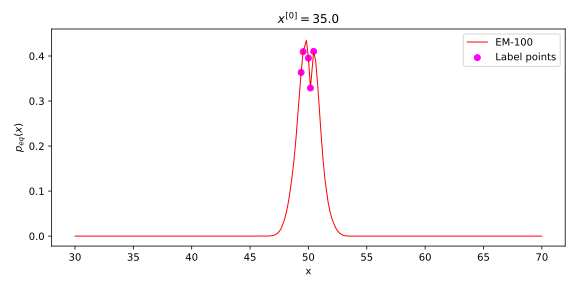
\includegraphics[scale=0.5]{ch4/abrupt_detect.pdf}   
\end{center}

\subsubsection{Step 2: The cubic smoothing spline}
\begin{definition}[Smoothing Spline]
    Let  $\{x_{i},Y_{i}:i=1,\dots ,n\}$ be a set of observations, modeled by the relation $\{Y_{i}=f(x_{i})+\epsilon _{i}\}$ where the $\epsilon _{i}$ are independen, zero mean random variables (usually assumed to have constant variance). The cubic smoothing spline estimate $\hat{f}$ of the function $f$ is defined to be the minimizer (over the class of twice differentiable functions) of
    \begin{equation}
         \sum _{i=1}^{n}\{Y_{i}-{\hat {f}}(x_{i})\}^{2}+\lambda \int {\hat {f}}''(x)^{2}\,dx
    \end{equation}
    \begin{itemize}
        \item $\lambda \geq 0$ is a smoothing parameter, controlling the trade-off between fidelity to the data and roughness of the function estimate. This is often estimated by generalized cross-validation, or by restricted marginal likelihood (REML) which exploits the link between spline smoothing and Bayesian estimation (the smoothing penalty can be viewed as being induced by a prior on the $f$.
        \item As $ \lambda \to 0$, the smoothing spline converges to the interpolating spline.
        \item As $\lambda \to \infty$(infinite smoothing), the roughness penalty becomes paramount and the estimate converges to a linear least squares estimate.
    \end{itemize}
\end{definition}
\begin{center}
    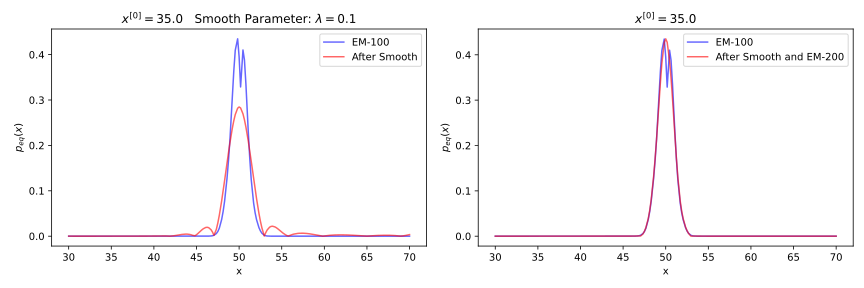
\includegraphics[scale=0.45]{ch4/double_peak_smooth_afterEM.pdf}   
\end{center}

\subsubsection{Result}
\begin{center}
    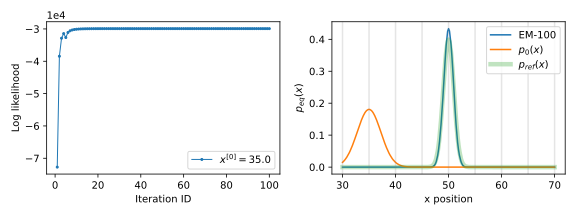
\includegraphics[scale=0.6]{ch4/aftersmooth_result.pdf}   
\end{center}

\section{Optimize diffusion coefficient D}
Here, we use the following simulation data to understand the procedure of updating D.
\begin{center}
    \includegraphics[scale=0.45]{ch4/Simu_for_EM.png}   
\end{center}
We will fix $p_{eq}^{[k]}$ as the real answer $p_{eq}$, and change $D$ to see the effect to eigenvalues $\lambda_i$ and log-likelihood $l[\theta]$

\subsection{Hamiltonian and its eigenvalues scale linearly with diffusion coefficient}
\begin{align*}
    \frac{\partial \rho(x,t)}{\partial t} &= -\bm{H}^0 \rho(x,t), \\
    \bm{H}^0 &= -D\nabla^2  + V_{\rm eff}(x), \\
    V_{\rm eff}  &= \frac{DF'(x)}{2} + \frac{DF^2(x)}{4}.
\end{align*}
\begin{center}
    \includegraphics[scale=0.45]{ch4/eigenvalue_linear_with_D.pdf}   
\end{center}
I only show the first six eigenvalues, all the rest eigenvalues is linear scaling with $D$.

\subsection{Log-likelihood as a function of D}
First, I try 
\begin{align*}
    D = 10^{m}~\si{\angstrom}^{2}s^{-1}\text{   where } m=-2,...,11
\end{align*}
\begin{center}
    \includegraphics[scale=0.45]{ch4/D_loglikelihood_broad_search.pdf} 
\end{center}
Then, focus on the range from $1 \times 10^{8}$ to $9 \times 10^{9}$
\begin{center}
    \includegraphics[scale=0.45]{ch4/D_loglikelihood_middle_search.pdf}   
\end{center}
At last, I focus on the range from $1.1 \times 10^{9}$ to $9.9 \times 10^{9}$
\begin{center}
    \includegraphics[scale=0.45]{ch4/D_loglikelihood_detail_search.pdf}   
\end{center}

\section{Complete EM}
\subsection{Initial Guess by Gaussian Kernel Density Estimation}
\begin{center}
    \includegraphics[scale=0.45]{ch4/Gaussian_Kde_harmonic_well.pdf} 
\end{center}

\subsection{Algorithm}
\begin{algorithm}[H]
    \SetAlgoLined
    \KwResult{$p^{k}_{\rm eq}$, $D^k$}
     initialize $p^0_{\rm eq}$ as Gaussian KDE \;
     initialize $D^0=\frac{k_B T}{6\pi \eta a}$\;
     
     \While{$(\ell[\theta^k] - \ell[\theta^{k-1}] > \num{1e-1})$ \& $(k < k_{\text{max}})$}{
       Eigen-decompose the Hermitian $\bm H$ for $\Psi$ and $\Lambda$\;
       Evaluate $\ell [\theta^k] = \sum_{\tau} |\alpha_{\tau}|$ via normalization\;
       Infer the latent states $\langle \alpha(t)|,|\beta(t) \rangle$\;
       Collect statistics of $\mathbb{E}^k_{X|Y}[a_ib_j] = \sum_{\tau}\Gamma^{\tau}_{ij}$\;
       Update $p_{\rm{eq}}^{k+1} = p^k_{\rm{eq}}(x) \sum_{ij} \mathbb{E}^k_{X|Y}[a_ib_j] \phi_i(x)\phi_j(x) $\;
       %
      \If{$k~\%~ 5 == 0$}{
       Detect abrupt change in $p^{k+1}_{\rm eq}$\;
       \If{abrupt change exists}{
           $p^{k+1}_{\rm eq}$ = Smooth($p^{k+1}_{\rm eq}$) 
       }
       Line search $D^{k+1} = \argmax_D \ell[p^{k+1}_{\rm eq},D]$\;
       }
       k = k + 1\;
     }
     \caption{Expectation-Maximization Statistical Learning for $F(x)$ and $D$}
\end{algorithm}

\subsection{The data strucutres for storing results}
\begin{align*}
    \mathrm{p\_container} &= 
    \begin{bmatrix}
        p^{0}_{\rm eq} \\ p^{1}_{\rm eq} \\ \vdots \\ p^{k}_{\rm eq}
    \end{bmatrix}\\
    \mathrm{D\_records} &= 
    \begin{bmatrix}
        D^{0} \\ D^{1} \\ \vdots \\ D^{k}
    \end{bmatrix}\\
    \mathrm{log\_likelihood\_records} &= 
    \begin{bmatrix}
        \ell[\theta^{0}] \\ \ell[\theta^{1}] \\ \vdots \\ \ell[\theta^{k}]
    \end{bmatrix}   
\end{align*}

\subsection{Results}
\begin{center}
    \includegraphics[scale=0.45]{ch4/em_p0_kde_pref_xavg_50.pdf} 
\end{center}

\section{Regularization by using Trajectory Entropy}
The proposed statistical learning problem of Langevin dynamics from smFRET data is naturally underdetermined because we attempt to extract a continuous profile from a finite number of photons. A Bayesian prior is thus required to break the degeneracy in the parameter set. With the prior, the posterior function, $p(\theta | \textbf{y})$, for parameter optimization becomes
\begin{equation}
    p(\theta | \textbf{y}) = \frac{p(\textbf{y}|\theta) p(\theta)}{p(\textbf{y})}
\end{equation}
A criterion for choosing the prior is to guide the optimization toward $F(x)$ profiles that imply the least amount information of dynamics. The goal is to prevent the statistical learning from overfitting and overinterpreting the measured data. As such, we selet the prior based on maximum trajectory entropy. For Langevin dynamics at equilibrium, the trajectory entropy is 
\begin{equation}
    \textbf{S}[F(x), D; D] = S_{\rm eq} - t_{\rm obs} \frac{D}{4}\left< F^2(x)\right>
\end{equation}
In Kevin's EM 2013 JPCB paper,
\begin{align}
    D &= 500~~\text{s}^{-1} \\
    \eta_{F} &= 2 \times 10^{-7} \\ 
    \eta_{F}D &= 0.0001
\end{align}
Therefore, when including the prior for updating $p_{\rm eq}$
\begin{align*}
    p_{\rm eq}^{k+1}(x) &= \left(\mathbb{E}^k_{X|Y} \left[\delta(x-X) \right]\right)^{1/(1+\eta_FD)} \\
    &= \left(\mathbb{E}^k_{X|Y} \left[\delta(x-X) \right]\right)^{1/(1+0.0001)} \\
    &= \left(\mathbb{E}^k_{X|Y} \left[\delta(x-X) \right]\right)^{1/(1.0001)}
\end{align*}
I think the regularization has no real effect.

\section{Double Well}
\subsection{Case 1: 10000 photons}
$\Delta t = 10^{-9}~\text{s}$
\begin{center}
    \includegraphics[scale=0.45]{ch4/simu_doublewell_10000photons.png} 
\end{center}
\begin{center}
    \includegraphics[scale=0.45]{ch4/em_p0_kde_pref_doublewell_10000photons.pdf} 
\end{center}

\subsection{Case 2: 20000 photons}
$\Delta t = 10^{-9}~\text{s}$
\begin{center}
    \includegraphics[scale=0.45]{ch4/simu_doublewell_20000photons.png} 
\end{center}
\begin{center}
    \includegraphics[scale=0.45]{ch4/em_p0_kde_pref_doublewell_20000photons.pdf} 
\end{center}

\subsection{Gaussian mixture model}
\begin{center}
    \includegraphics[scale=0.45]{ch4/gmm_doublewell_1.png} 
\end{center}
\begin{center}
    \includegraphics[scale=0.45]{ch4/em_p0_kde_pref_gmm_doublewell_1.pdf} 
\end{center}

\section{Triple Well}
\subsection{Gaussian mixture model: 10000 photons}
\begin{center}
    \includegraphics[scale=0.45]{ch4/gmm_triplewell_1.png} 
\end{center}
\begin{center}
    \includegraphics[scale=0.45]{ch4/em_p0_kde_pref_gmm_triplewell_1.pdf} 
\end{center}

\subsection{Gaussian mixture model: 50000 photons}
\begin{center}
    \includegraphics[scale=0.45]{ch4/gmm_triplewell_2.png} 
\end{center}
\begin{center}
    \includegraphics[scale=0.45]{ch4/em_p0_kde_pref_gmm_triplewell_2.pdf} 
\end{center}


\end{document}